% Options for packages loaded elsewhere
\PassOptionsToPackage{unicode}{hyperref}
\PassOptionsToPackage{hyphens}{url}
%
\documentclass[
]{article}
\usepackage{amsmath,amssymb}
\usepackage{iftex}
\ifPDFTeX
  \usepackage[T1]{fontenc}
  \usepackage[utf8]{inputenc}
  \usepackage{textcomp} % provide euro and other symbols
\else % if luatex or xetex
  \usepackage{unicode-math} % this also loads fontspec
  \defaultfontfeatures{Scale=MatchLowercase}
  \defaultfontfeatures[\rmfamily]{Ligatures=TeX,Scale=1}
\fi
\usepackage{lmodern}
\ifPDFTeX\else
  % xetex/luatex font selection
\fi
% Use upquote if available, for straight quotes in verbatim environments
\IfFileExists{upquote.sty}{\usepackage{upquote}}{}
\IfFileExists{microtype.sty}{% use microtype if available
  \usepackage[]{microtype}
  \UseMicrotypeSet[protrusion]{basicmath} % disable protrusion for tt fonts
}{}
\makeatletter
\@ifundefined{KOMAClassName}{% if non-KOMA class
  \IfFileExists{parskip.sty}{%
    \usepackage{parskip}
  }{% else
    \setlength{\parindent}{0pt}
    \setlength{\parskip}{6pt plus 2pt minus 1pt}}
}{% if KOMA class
  \KOMAoptions{parskip=half}}
\makeatother
\usepackage{xcolor}
\usepackage[margin=1in]{geometry}
\usepackage{color}
\usepackage{fancyvrb}
\newcommand{\VerbBar}{|}
\newcommand{\VERB}{\Verb[commandchars=\\\{\}]}
\DefineVerbatimEnvironment{Highlighting}{Verbatim}{commandchars=\\\{\}}
% Add ',fontsize=\small' for more characters per line
\usepackage{framed}
\definecolor{shadecolor}{RGB}{248,248,248}
\newenvironment{Shaded}{\begin{snugshade}}{\end{snugshade}}
\newcommand{\AlertTok}[1]{\textcolor[rgb]{0.94,0.16,0.16}{#1}}
\newcommand{\AnnotationTok}[1]{\textcolor[rgb]{0.56,0.35,0.01}{\textbf{\textit{#1}}}}
\newcommand{\AttributeTok}[1]{\textcolor[rgb]{0.13,0.29,0.53}{#1}}
\newcommand{\BaseNTok}[1]{\textcolor[rgb]{0.00,0.00,0.81}{#1}}
\newcommand{\BuiltInTok}[1]{#1}
\newcommand{\CharTok}[1]{\textcolor[rgb]{0.31,0.60,0.02}{#1}}
\newcommand{\CommentTok}[1]{\textcolor[rgb]{0.56,0.35,0.01}{\textit{#1}}}
\newcommand{\CommentVarTok}[1]{\textcolor[rgb]{0.56,0.35,0.01}{\textbf{\textit{#1}}}}
\newcommand{\ConstantTok}[1]{\textcolor[rgb]{0.56,0.35,0.01}{#1}}
\newcommand{\ControlFlowTok}[1]{\textcolor[rgb]{0.13,0.29,0.53}{\textbf{#1}}}
\newcommand{\DataTypeTok}[1]{\textcolor[rgb]{0.13,0.29,0.53}{#1}}
\newcommand{\DecValTok}[1]{\textcolor[rgb]{0.00,0.00,0.81}{#1}}
\newcommand{\DocumentationTok}[1]{\textcolor[rgb]{0.56,0.35,0.01}{\textbf{\textit{#1}}}}
\newcommand{\ErrorTok}[1]{\textcolor[rgb]{0.64,0.00,0.00}{\textbf{#1}}}
\newcommand{\ExtensionTok}[1]{#1}
\newcommand{\FloatTok}[1]{\textcolor[rgb]{0.00,0.00,0.81}{#1}}
\newcommand{\FunctionTok}[1]{\textcolor[rgb]{0.13,0.29,0.53}{\textbf{#1}}}
\newcommand{\ImportTok}[1]{#1}
\newcommand{\InformationTok}[1]{\textcolor[rgb]{0.56,0.35,0.01}{\textbf{\textit{#1}}}}
\newcommand{\KeywordTok}[1]{\textcolor[rgb]{0.13,0.29,0.53}{\textbf{#1}}}
\newcommand{\NormalTok}[1]{#1}
\newcommand{\OperatorTok}[1]{\textcolor[rgb]{0.81,0.36,0.00}{\textbf{#1}}}
\newcommand{\OtherTok}[1]{\textcolor[rgb]{0.56,0.35,0.01}{#1}}
\newcommand{\PreprocessorTok}[1]{\textcolor[rgb]{0.56,0.35,0.01}{\textit{#1}}}
\newcommand{\RegionMarkerTok}[1]{#1}
\newcommand{\SpecialCharTok}[1]{\textcolor[rgb]{0.81,0.36,0.00}{\textbf{#1}}}
\newcommand{\SpecialStringTok}[1]{\textcolor[rgb]{0.31,0.60,0.02}{#1}}
\newcommand{\StringTok}[1]{\textcolor[rgb]{0.31,0.60,0.02}{#1}}
\newcommand{\VariableTok}[1]{\textcolor[rgb]{0.00,0.00,0.00}{#1}}
\newcommand{\VerbatimStringTok}[1]{\textcolor[rgb]{0.31,0.60,0.02}{#1}}
\newcommand{\WarningTok}[1]{\textcolor[rgb]{0.56,0.35,0.01}{\textbf{\textit{#1}}}}
\usepackage{graphicx}
\makeatletter
\def\maxwidth{\ifdim\Gin@nat@width>\linewidth\linewidth\else\Gin@nat@width\fi}
\def\maxheight{\ifdim\Gin@nat@height>\textheight\textheight\else\Gin@nat@height\fi}
\makeatother
% Scale images if necessary, so that they will not overflow the page
% margins by default, and it is still possible to overwrite the defaults
% using explicit options in \includegraphics[width, height, ...]{}
\setkeys{Gin}{width=\maxwidth,height=\maxheight,keepaspectratio}
% Set default figure placement to htbp
\makeatletter
\def\fps@figure{htbp}
\makeatother
\setlength{\emergencystretch}{3em} % prevent overfull lines
\providecommand{\tightlist}{%
  \setlength{\itemsep}{0pt}\setlength{\parskip}{0pt}}
\setcounter{secnumdepth}{-\maxdimen} % remove section numbering
\ifLuaTeX
  \usepackage{selnolig}  % disable illegal ligatures
\fi
\IfFileExists{bookmark.sty}{\usepackage{bookmark}}{\usepackage{hyperref}}
\IfFileExists{xurl.sty}{\usepackage{xurl}}{} % add URL line breaks if available
\urlstyle{same}
\hypersetup{
  pdftitle={Métodos Cuantitativos en Ecología - MCE5},
  pdfauthor={David Grefa},
  hidelinks,
  pdfcreator={LaTeX via pandoc}}

\title{Métodos Cuantitativos en Ecología - MCE5}
\usepackage{etoolbox}
\makeatletter
\providecommand{\subtitle}[1]{% add subtitle to \maketitle
  \apptocmd{\@title}{\par {\large #1 \par}}{}{}
}
\makeatother
\subtitle{EXAMEN FINAL - 2022II}
\author{David Grefa}
\date{2023-07-11}

\begin{document}
\maketitle

{
\setcounter{tocdepth}{4}
\tableofcontents
}
Los contenidos de esta evaluación corresponden a los temas:

\begin{itemize}
\item
  GLM y GAM
\item
  Introducción a estadística Bayesiana
\item
  Series de tiempo
\item
  Análisis espacial
\end{itemize}

Ustedes estan utilizando un archivo tipo R Markdown (\texttt{.Rmd}). Las
instruciones son \textbf{{[}1 PUNTO{]}}:

\begin{itemize}
\item
  Bifurquen el repositorio en GitHub y clonen en su computador usando un
  proyecto con control de la versión de RStudio.
\item
  Arriba, donde dice ``author'', deben llenar sus nombres.
\item
  \textbf{Todo resultado debe ir con su explicación y/o discusión, caso
  contrario no se calificará.}
\item
  \textbf{NO IMPRIMA los datos o tablas completas}, reporte únicamente
  figuras o tablas resumen. Si tiene varias figuras use la función
  \texttt{ggarrange} de la librería \texttt{ggpubr}.
\item
  Al final de este examen deben utilizar el comando ``Knit'' para
  generar un archivo HTML.
\item
  \textbf{Cada pregunta debe tener al menos un cntrol de la versión}.
\item
  Su entrega consiste en colocar el \textbf{enlace de GitHub} en la
  actividad ``ExamenFinal''.
\end{itemize}

\hypertarget{pregunta-1-glm-gam-y-regresiuxf3n-bayesiana-3-puntos}{%
\subsection{\texorpdfstring{\textbf{PREGUNTA 1: GLM, GAM y Regresión
Bayesiana {[}3
PUNTOS{]}}}{PREGUNTA 1: GLM, GAM y Regresión Bayesiana {[}3 PUNTOS{]}}}\label{pregunta-1-glm-gam-y-regresiuxf3n-bayesiana-3-puntos}}

En el archivo \texttt{"glm.xlsx"} tiene tres datos:

\begin{itemize}
\item
  aedes: insecticidas utilizados para controlar el número de mosquitos
  en un experimento. Cada vez que se repite la aplicación del
  insecticida parece disminuir la cantidad de zancudos vivos.
\item
  leishmania: en una infección con leishmania cuando se analiza el
  tejido qué sucede con la concentración de algunas células y si están o
  no afectadas.
\item
  disease: cómo la edad afecta a diferentes características dicotómicas.
\end{itemize}

Realice los siguientes análisis:

\begin{itemize}
\item
  aedes: GLM Poisson
\item
  disease: GLMs binomiales
\item
  leishmania: glm bayesiano
\end{itemize}

Realizar los siguientes análisis y respectivas interpretaciones:

\begin{enumerate}
\def\labelenumi{\arabic{enumi}.}
\item
  Análisis exploratorio.
\item
  Planteamiento de hipótesis.
\item
  Análisis de regresión
\item
  Planteamiento del modelo.
\item
  Validez del modelo.
\end{enumerate}

\#1\_Análisis exploratorio

\begin{Shaded}
\begin{Highlighting}[]
\FunctionTok{library}\NormalTok{(readxl)}
\NormalTok{glm }\OtherTok{\textless{}{-}} \FunctionTok{read\_excel}\NormalTok{(}\StringTok{"glm.xlsx"}\NormalTok{)}
\FunctionTok{View}\NormalTok{(glm)}
\FunctionTok{head}\NormalTok{(glm)}
\end{Highlighting}
\end{Shaded}

\begin{verbatim}
## # A tibble: 6 x 3
##   agrochem repetition aedes
##   <chr>         <dbl> <dbl>
## 1 A                 1  2370
## 2 B                 1  1282
## 3 C                 1   562
## 4 D                 1   173
## 5 E                 1   193
## 6 A                 2  1687
\end{verbatim}

\begin{Shaded}
\begin{Highlighting}[]
\FunctionTok{str}\NormalTok{(glm)}
\end{Highlighting}
\end{Shaded}

\begin{verbatim}
## tibble [30 x 3] (S3: tbl_df/tbl/data.frame)
##  $ agrochem  : chr [1:30] "A" "B" "C" "D" ...
##  $ repetition: num [1:30] 1 1 1 1 1 2 2 2 2 2 ...
##  $ aedes     : num [1:30] 2370 1282 562 173 193 ...
\end{verbatim}

\begin{Shaded}
\begin{Highlighting}[]
\FunctionTok{summary}\NormalTok{(glm)}
\end{Highlighting}
\end{Shaded}

\begin{verbatim}
##    agrochem           repetition      aedes       
##  Length:30          Min.   :1.0   Min.   :  44.0  
##  Class :character   1st Qu.:2.0   1st Qu.: 136.5  
##  Mode  :character   Median :3.5   Median : 523.5  
##                     Mean   :3.5   Mean   : 865.4  
##                     3rd Qu.:5.0   3rd Qu.:1217.8  
##                     Max.   :6.0   Max.   :3020.0
\end{verbatim}

\textbf{descripción} Se realizó un análisis exploratorio de la data glm,
esta data contiene información de insecticidas para controlar el número
de mosquitos, donde se cargo la data, se usó la librería readxl, con
view(glm) se visualizó la información, head(glm) para visualizar los
primeros 6 datos, str(glm) para viszualizar si las variables son
numéricas o categóricas. \#2\_Planteamiento de hipótesis para cada
modelo

\textbf{hipótesis}la Aplicación repetida de insecticidas en un
experimento para controlar el número de mosquitos de Aedes reduce
efectivamente su población.a.

\textbf{Hipótesis}: La edad tiene un efecto en la presencia o ausencia
de las variables

\textbf{Hipótesis}: Las variables relacionadas con la concentración y
afectación de ciertas células se relacionan con la presencia/ausencia de
infección causad por leishmania.

\#3\_Análisis de regresión para aedes, leishmania, disease

\#Análisis GLM poisson en aedes

\begin{Shaded}
\begin{Highlighting}[]
\NormalTok{glm }\OtherTok{\textless{}{-}} \FunctionTok{read\_excel}\NormalTok{(}\StringTok{"glm.xlsx"}\NormalTok{, }\AttributeTok{sheet =} \StringTok{"aedes"}\NormalTok{)}

\CommentTok{\# Convertir la variable a factor}
\NormalTok{glm}\SpecialCharTok{$}\NormalTok{agrochem }\OtherTok{\textless{}{-}} \FunctionTok{factor}\NormalTok{(glm}\SpecialCharTok{$}\NormalTok{agrochem)}

\CommentTok{\# Realizar el análisis GLM Poisson}
\NormalTok{glm\_poisson\_model }\OtherTok{\textless{}{-}} \FunctionTok{glm}\NormalTok{(aedes }\SpecialCharTok{\textasciitilde{}}\NormalTok{ agrochem }\SpecialCharTok{+}\NormalTok{ repetition, }\AttributeTok{data =}\NormalTok{ glm, }\AttributeTok{family =}\NormalTok{ poisson)}
\FunctionTok{summary}\NormalTok{(glm\_poisson\_model)}
\end{Highlighting}
\end{Shaded}

\begin{verbatim}
## 
## Call:
## glm(formula = aedes ~ agrochem + repetition, family = poisson, 
##     data = glm)
## 
## Coefficients:
##              Estimate Std. Error z value Pr(>|z|)    
## (Intercept)  7.720708   0.015380 502.008  < 2e-16 ***
## agrochemB   -0.834727   0.014911 -55.982  < 2e-16 ***
## agrochemC   -1.547287   0.019582 -79.017  < 2e-16 ***
## agrochemD   -2.762813   0.033666 -82.066  < 2e-16 ***
## agrochemE   -3.300288   0.043497 -75.873  < 2e-16 ***
## repetition   0.026590   0.003636   7.312 2.63e-13 ***
## ---
## Signif. codes:  0 '***' 0.001 '**' 0.01 '*' 0.05 '.' 0.1 ' ' 1
## 
## (Dispersion parameter for poisson family taken to be 1)
## 
##     Null deviance: 26630.9  on 29  degrees of freedom
## Residual deviance:  1329.9  on 24  degrees of freedom
## AIC: 1579.4
## 
## Number of Fisher Scoring iterations: 4
\end{verbatim}

\begin{Shaded}
\begin{Highlighting}[]
\CommentTok{\# Visualizar los coeficientes estimados del modelo}
\FunctionTok{coef}\NormalTok{(glm\_poisson\_model)}
\end{Highlighting}
\end{Shaded}

\begin{verbatim}
## (Intercept)   agrochemB   agrochemC   agrochemD   agrochemE  repetition 
##  7.72070788 -0.83472749 -1.54728668 -2.76281295 -3.30028761  0.02658992
\end{verbatim}

\begin{Shaded}
\begin{Highlighting}[]
\FunctionTok{print}\NormalTok{(glm\_poisson\_model)}
\end{Highlighting}
\end{Shaded}

\begin{verbatim}
## 
## Call:  glm(formula = aedes ~ agrochem + repetition, family = poisson, 
##     data = glm)
## 
## Coefficients:
## (Intercept)    agrochemB    agrochemC    agrochemD    agrochemE   repetition  
##     7.72071     -0.83473     -1.54729     -2.76281     -3.30029      0.02659  
## 
## Degrees of Freedom: 29 Total (i.e. Null);  24 Residual
## Null Deviance:       26630 
## Residual Deviance: 1330  AIC: 1579
\end{verbatim}

\begin{Shaded}
\begin{Highlighting}[]
\CommentTok{\#vizualización }
\FunctionTok{plot}\NormalTok{(glm\_poisson\_model)}
\end{Highlighting}
\end{Shaded}

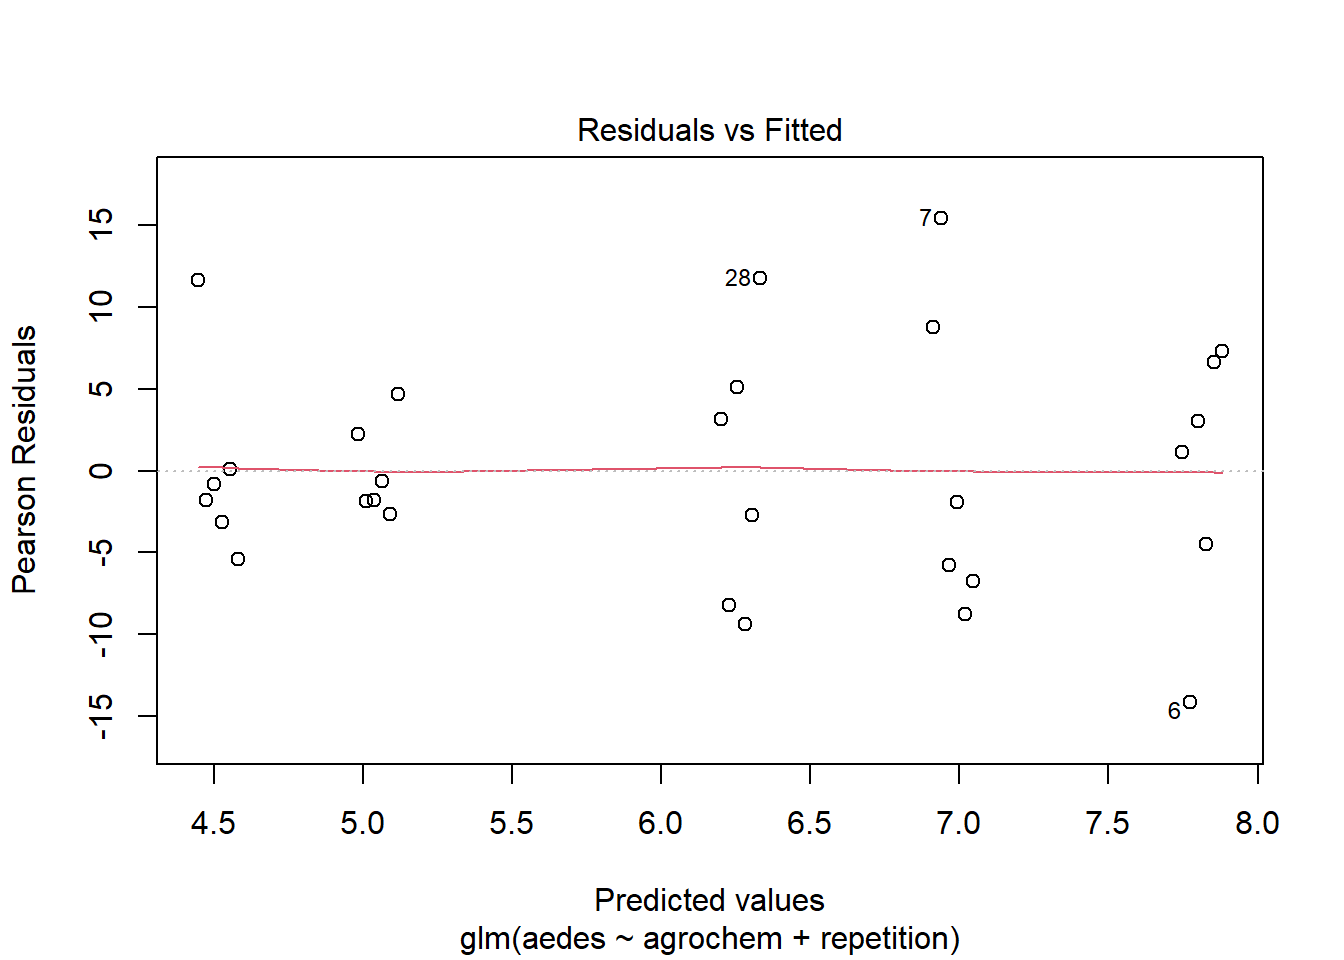
\includegraphics{2022II_MCE5_ExamenFinal_files/figure-latex/unnamed-chunk-2-1.pdf}
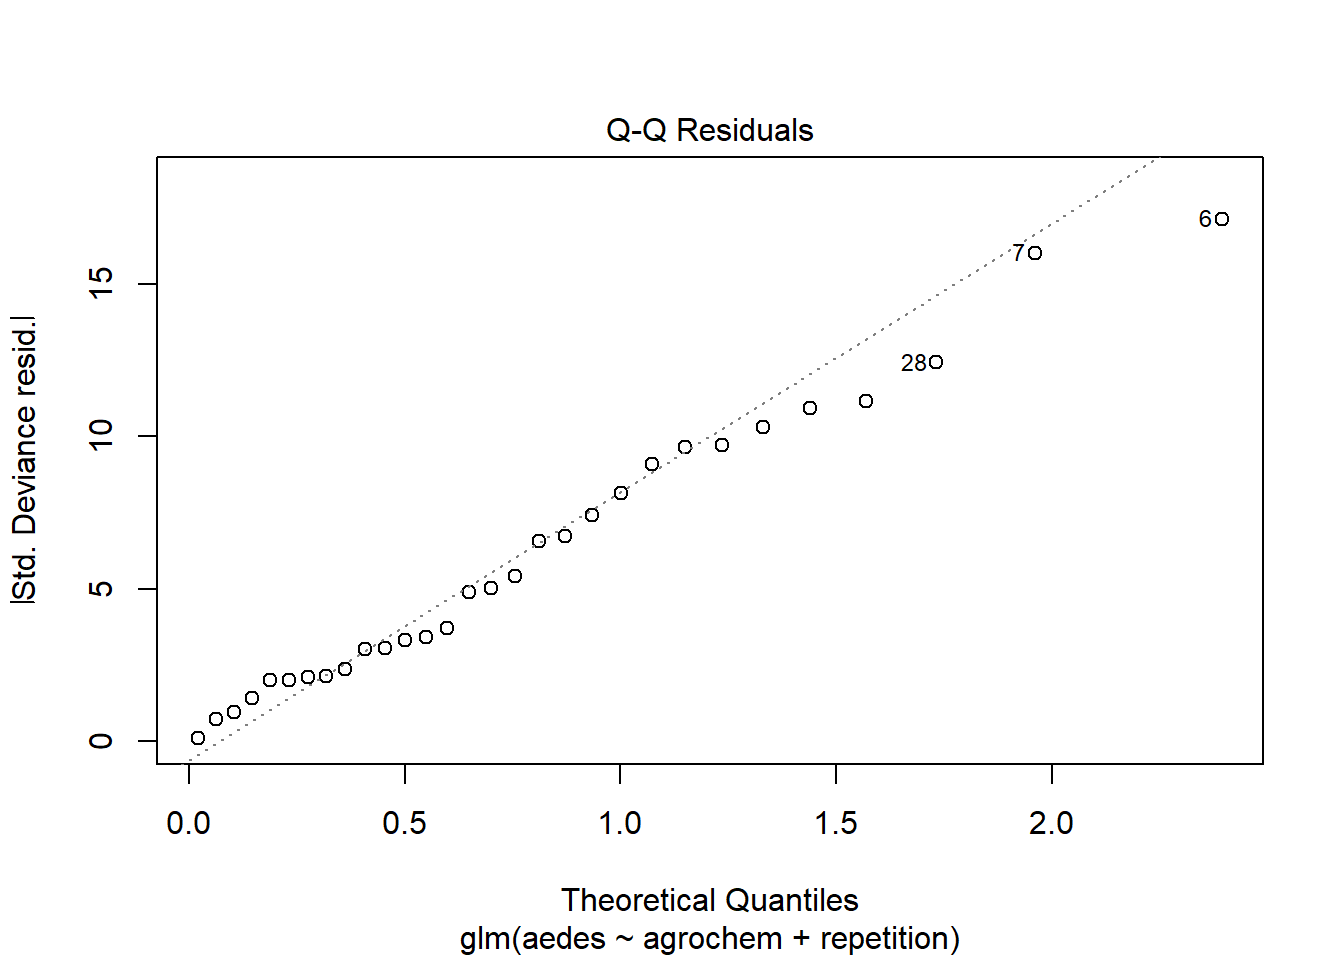
\includegraphics{2022II_MCE5_ExamenFinal_files/figure-latex/unnamed-chunk-2-2.pdf}
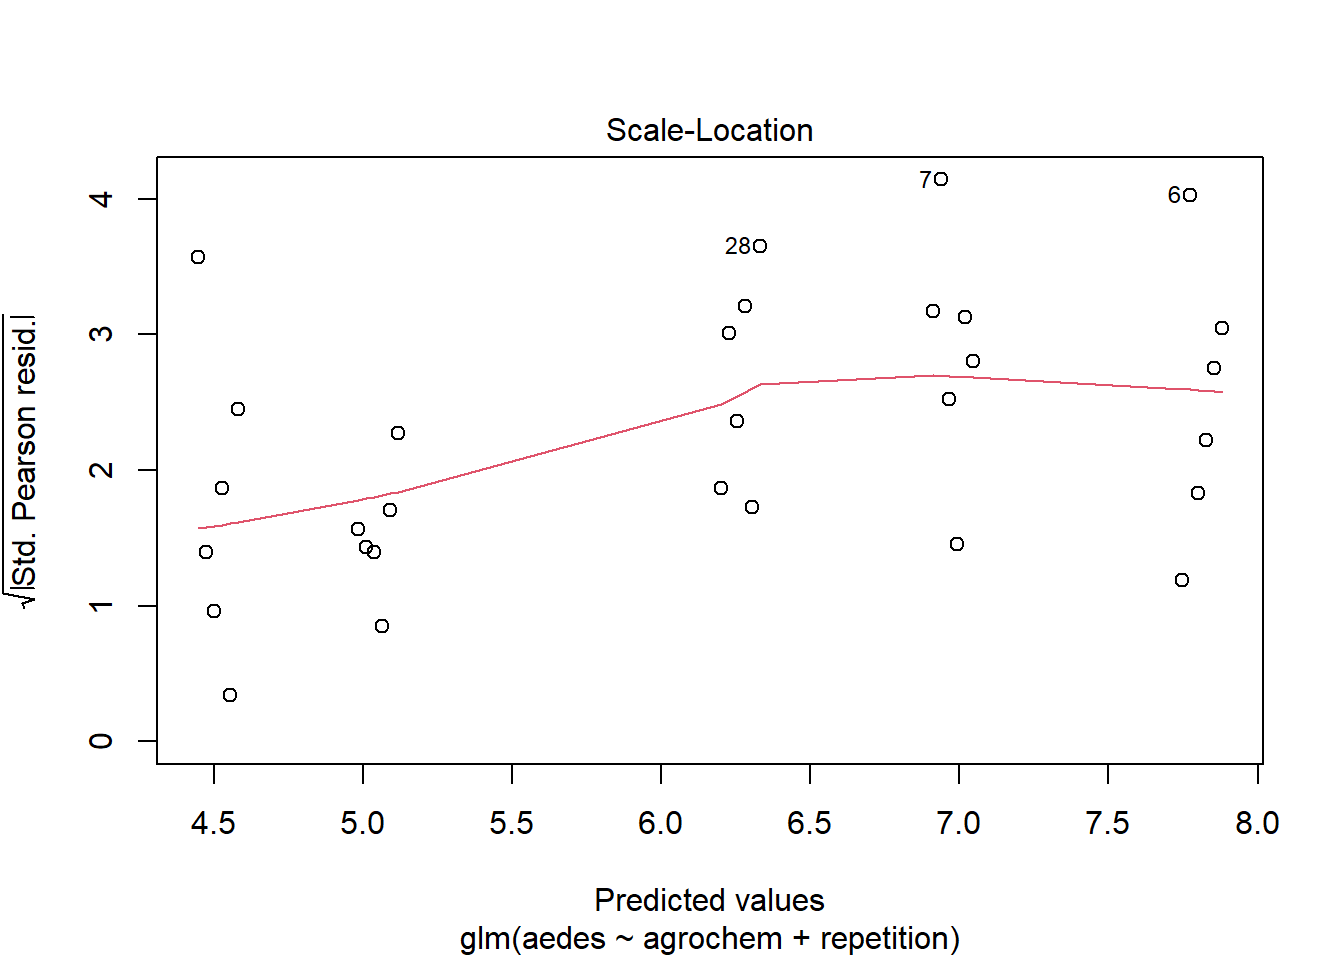
\includegraphics{2022II_MCE5_ExamenFinal_files/figure-latex/unnamed-chunk-2-3.pdf}
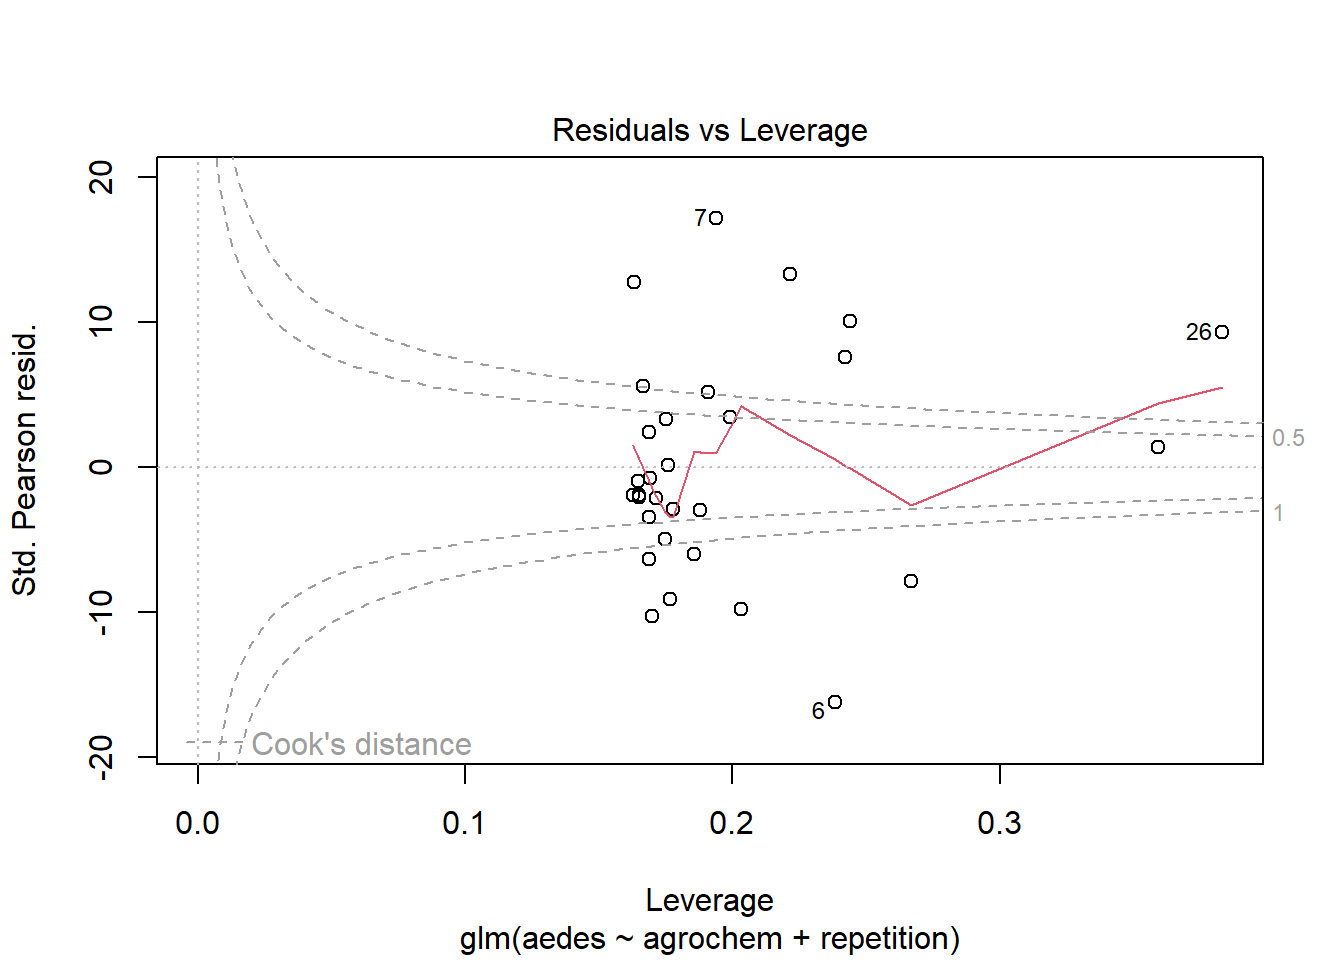
\includegraphics{2022II_MCE5_ExamenFinal_files/figure-latex/unnamed-chunk-2-4.pdf}
\textbf{Descripción} la variable agroquimica tiene efecto significativo
en la variable de respuesta. Los todos los niveles de los
agroquimicos,se relacionan con la disminucion en la cantidad de
mosquitos con el nivel A, mientras mas repeticiones hay se reduce el
número demoquitos

\#Análisis GLMs binomiales en disease

\begin{Shaded}
\begin{Highlighting}[]
\NormalTok{glm\_disease }\OtherTok{\textless{}{-}} \FunctionTok{read\_excel}\NormalTok{(}\StringTok{"glm.xlsx"}\NormalTok{, }\AttributeTok{sheet =} \StringTok{"disease"}\NormalTok{)}
\FunctionTok{View}\NormalTok{(glm)}

\CommentTok{\# Convertir la variable a  factor}
\NormalTok{glm\_disease}\SpecialCharTok{$}\NormalTok{recover }\OtherTok{\textless{}{-}} \FunctionTok{factor}\NormalTok{(glm\_disease}\SpecialCharTok{$}\NormalTok{recover)}

\CommentTok{\# Realizar el análisis GLM binomial}
\NormalTok{glm\_binomial\_model }\OtherTok{\textless{}{-}} \FunctionTok{glm}\NormalTok{(recover }\SpecialCharTok{\textasciitilde{}}\NormalTok{ native }\SpecialCharTok{+}\NormalTok{ gender }\SpecialCharTok{+}\NormalTok{ treatment }\SpecialCharTok{+}\NormalTok{ age, }\AttributeTok{data =}\NormalTok{ glm\_disease, }\AttributeTok{family =}\NormalTok{ binomial)}

\FunctionTok{summary}\NormalTok{(glm\_binomial\_model)}
\end{Highlighting}
\end{Shaded}

\begin{verbatim}
## 
## Call:
## glm(formula = recover ~ native + gender + treatment + age, family = binomial, 
##     data = glm_disease)
## 
## Coefficients:
##             Estimate Std. Error z value Pr(>|z|)    
## (Intercept) -2.31293    0.64259  -3.599 0.000319 ***
## native       0.40879    0.59900   0.682 0.494954    
## gender      -0.30525    0.60413  -0.505 0.613362    
## treatment    1.57475    0.50162   3.139 0.001693 ** 
## age          0.02975    0.01350   2.203 0.027577 *  
## ---
## Signif. codes:  0 '***' 0.001 '**' 0.01 '*' 0.05 '.' 0.1 ' ' 1
## 
## (Dispersion parameter for binomial family taken to be 1)
## 
##     Null deviance: 122.32  on 97  degrees of freedom
## Residual deviance: 101.05  on 93  degrees of freedom
## AIC: 111.05
## 
## Number of Fisher Scoring iterations: 4
\end{verbatim}

\begin{Shaded}
\begin{Highlighting}[]
\CommentTok{\# Visualizar los coeficientes estimados del modelo}
\FunctionTok{coef}\NormalTok{(glm\_binomial\_model)}
\end{Highlighting}
\end{Shaded}

\begin{verbatim}
## (Intercept)      native      gender   treatment         age 
## -2.31293482  0.40879024 -0.30525456  1.57474923  0.02975009
\end{verbatim}

\begin{Shaded}
\begin{Highlighting}[]
\FunctionTok{print}\NormalTok{(glm\_binomial\_model)}
\end{Highlighting}
\end{Shaded}

\begin{verbatim}
## 
## Call:  glm(formula = recover ~ native + gender + treatment + age, family = binomial, 
##     data = glm_disease)
## 
## Coefficients:
## (Intercept)       native       gender    treatment          age  
##    -2.31293      0.40879     -0.30525      1.57475      0.02975  
## 
## Degrees of Freedom: 97 Total (i.e. Null);  93 Residual
## Null Deviance:       122.3 
## Residual Deviance: 101.1     AIC: 111.1
\end{verbatim}

\begin{Shaded}
\begin{Highlighting}[]
\FunctionTok{plot}\NormalTok{(glm\_binomial\_model)}
\end{Highlighting}
\end{Shaded}

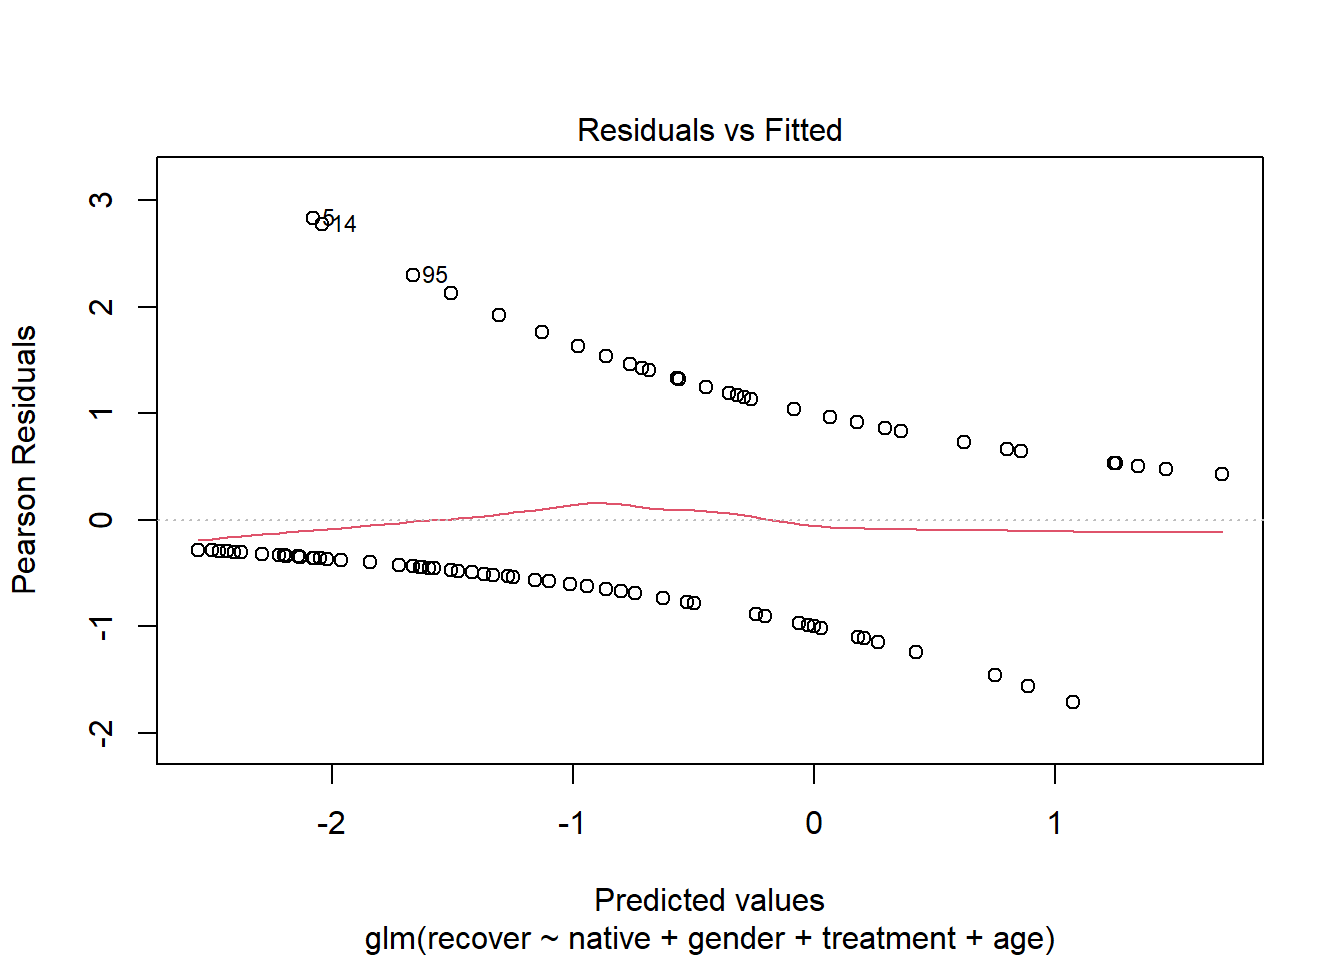
\includegraphics{2022II_MCE5_ExamenFinal_files/figure-latex/unnamed-chunk-3-1.pdf}
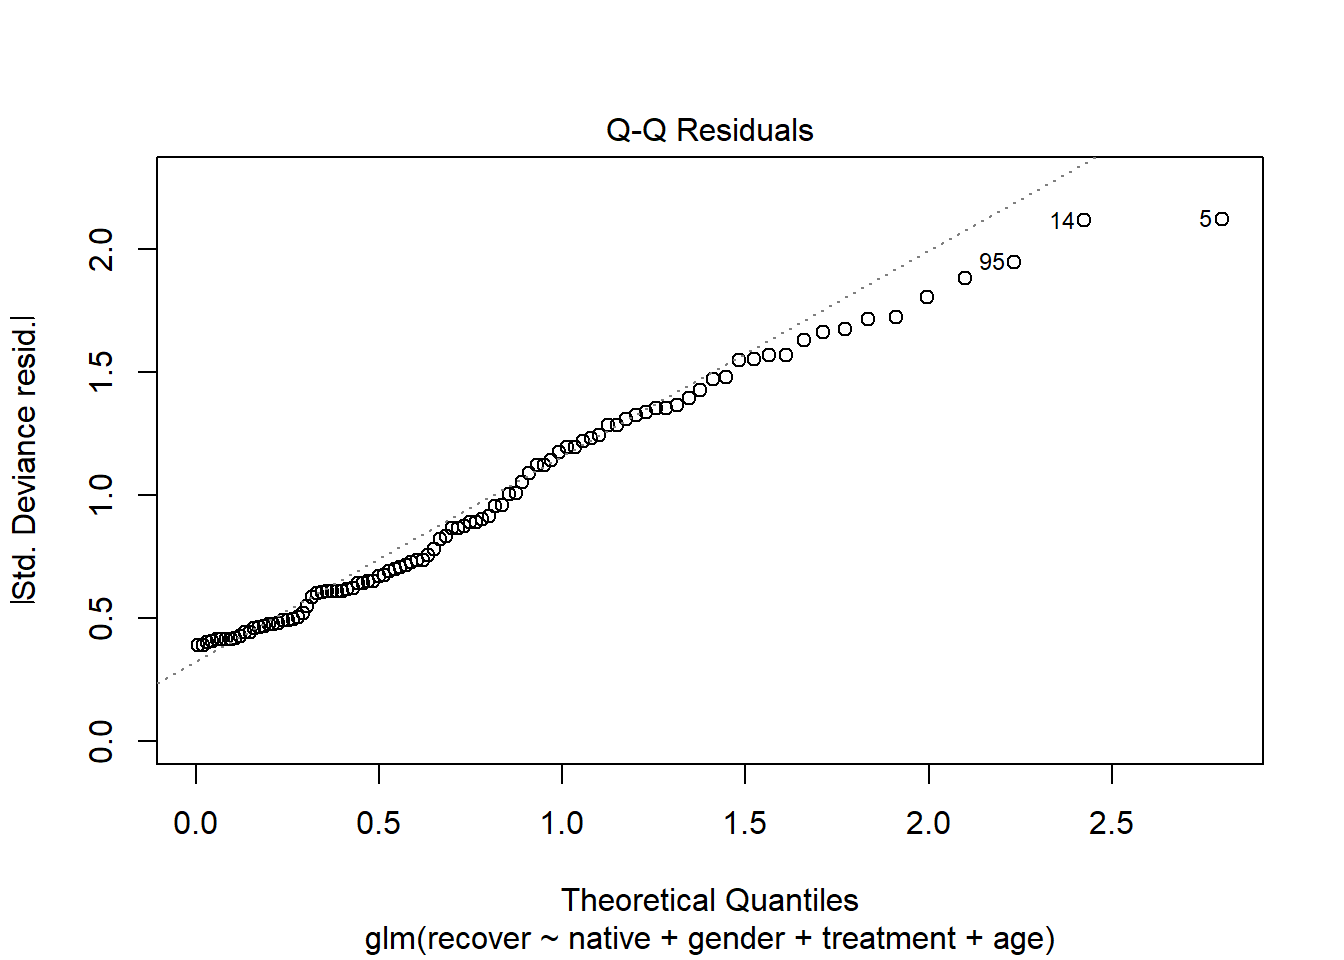
\includegraphics{2022II_MCE5_ExamenFinal_files/figure-latex/unnamed-chunk-3-2.pdf}
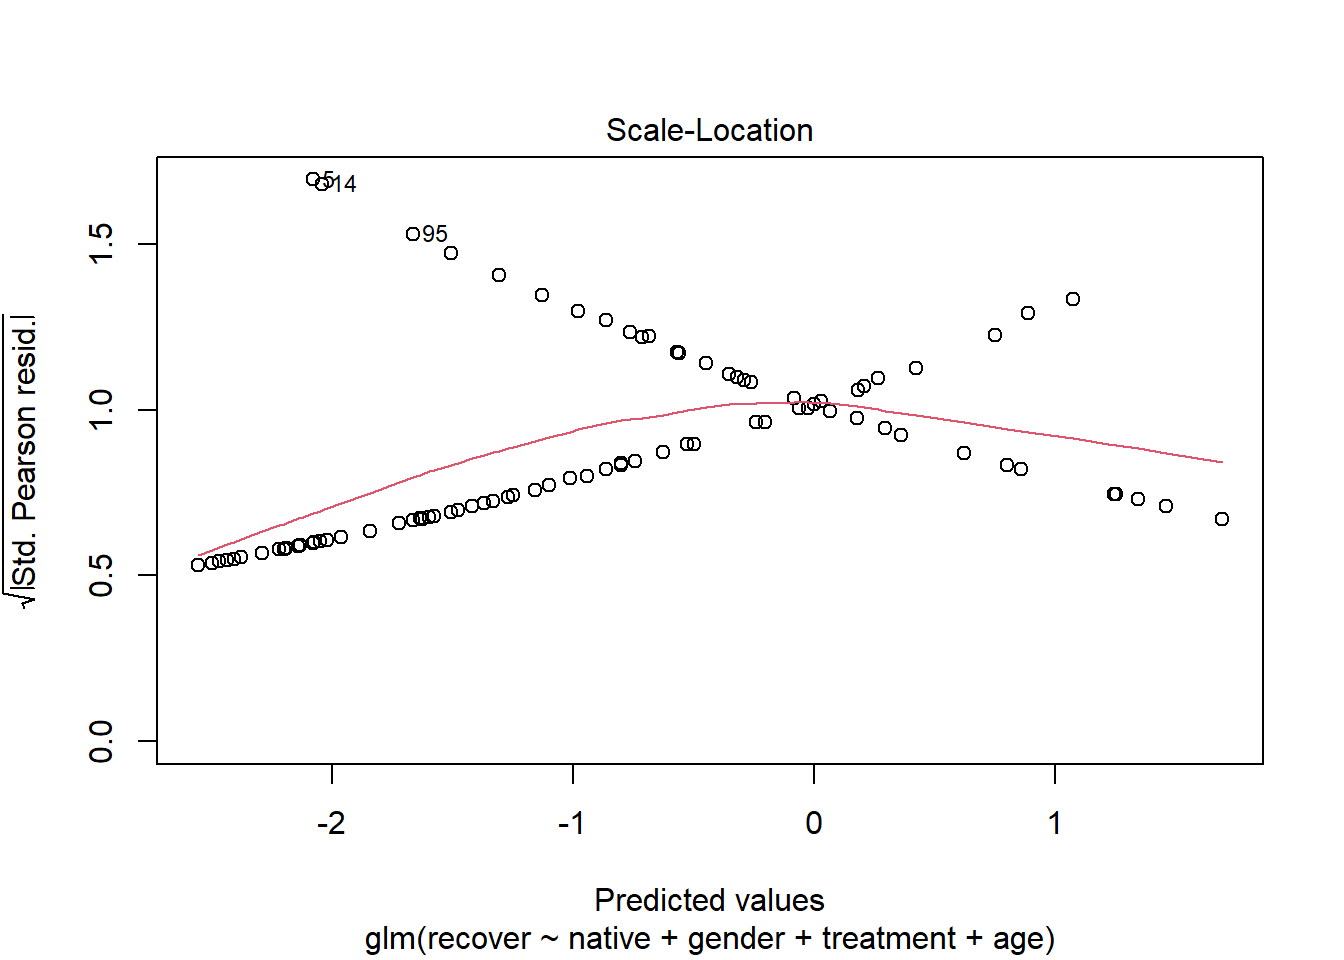
\includegraphics{2022II_MCE5_ExamenFinal_files/figure-latex/unnamed-chunk-3-3.pdf}
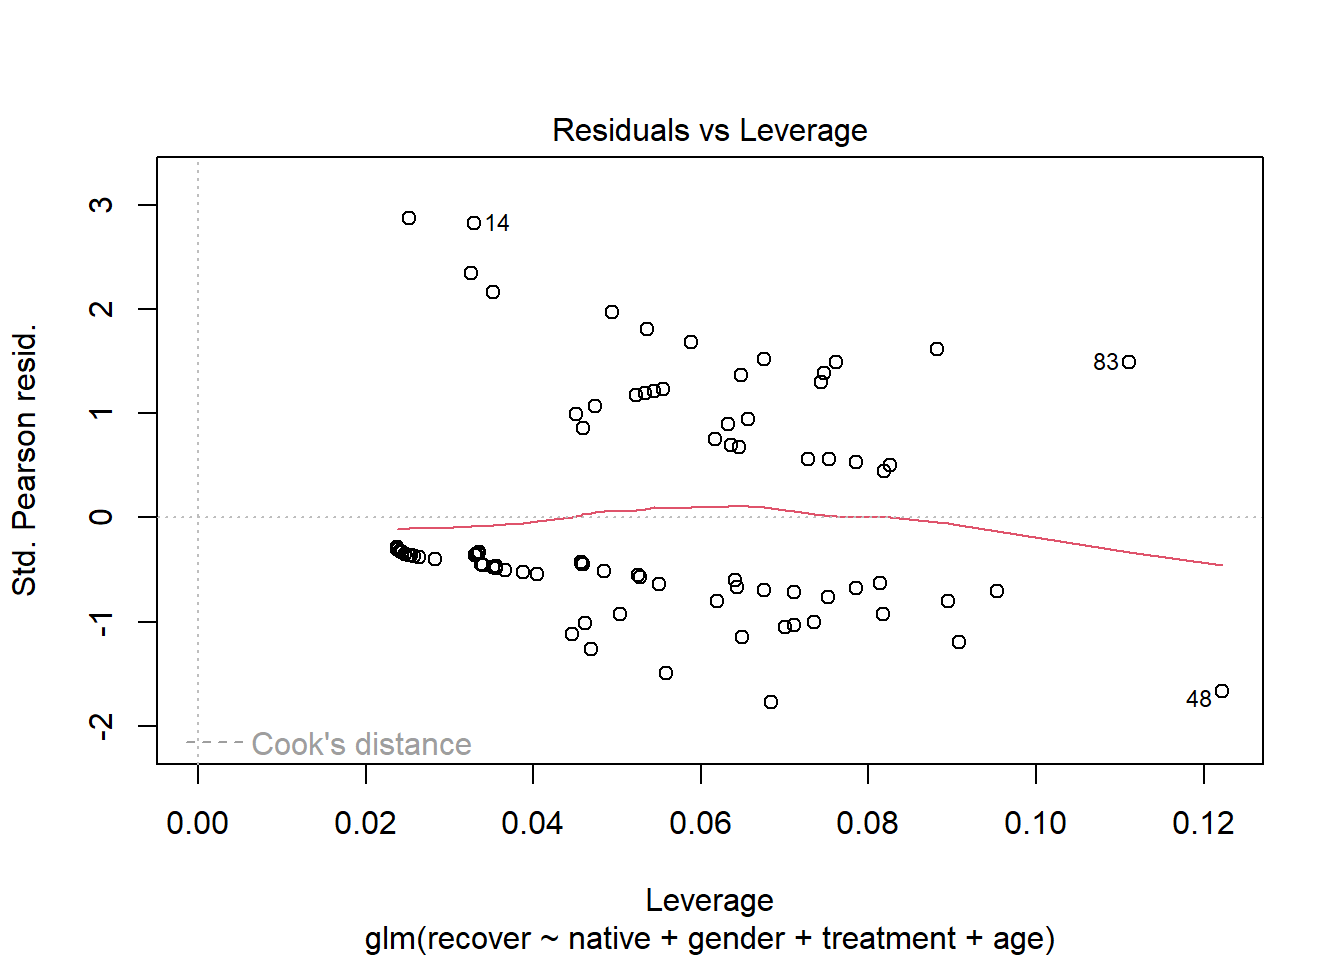
\includegraphics{2022II_MCE5_ExamenFinal_files/figure-latex/unnamed-chunk-3-4.pdf}
\textbf{descripción} Las variables ``native'', ``gender'', ``treatment''
y ``age'' tienen efectos diferentes en la variable de respuesta
``recover''. El intercepto muestra una menor probabilidad de
recuperación en ausencia de otras variables predictoras. El tratamiento
se asocia con una mayor probabilidad de recuperación, mientras que la
edad también influye de forma positiva enn en esta probabilidad.

\#Análisis bayesiano para leishmania

\begin{Shaded}
\begin{Highlighting}[]
\FunctionTok{library}\NormalTok{(rstanarm)}
\end{Highlighting}
\end{Shaded}

\begin{verbatim}
## Loading required package: Rcpp
\end{verbatim}

\begin{verbatim}
## This is rstanarm version 2.21.4
\end{verbatim}

\begin{verbatim}
## - See https://mc-stan.org/rstanarm/articles/priors for changes to default priors!
\end{verbatim}

\begin{verbatim}
## - Default priors may change, so it's safest to specify priors, even if equivalent to the defaults.
\end{verbatim}

\begin{verbatim}
## - For execution on a local, multicore CPU with excess RAM we recommend calling
\end{verbatim}

\begin{verbatim}
##   options(mc.cores = parallel::detectCores())
\end{verbatim}

\begin{Shaded}
\begin{Highlighting}[]
\NormalTok{glm\_leishmania }\OtherTok{\textless{}{-}} \FunctionTok{read\_excel}\NormalTok{(}\StringTok{"glm.xlsx"}\NormalTok{, }\AttributeTok{sheet =} \StringTok{"leishmania"}\NormalTok{)}
\FunctionTok{View}\NormalTok{(glm\_leishmania)}

\CommentTok{\# Realizar el análisis GLM bayesiano}
\NormalTok{bayesian\_glm\_model }\OtherTok{\textless{}{-}} \FunctionTok{stan\_glm}\NormalTok{(recupera }\SpecialCharTok{\textasciitilde{}}\NormalTok{ percent\_blast }\SpecialCharTok{+}\NormalTok{ percent\_affect }\SpecialCharTok{+}\NormalTok{ percent\_leuco }\SpecialCharTok{+}\NormalTok{ periferia\_leuco }\SpecialCharTok{+}\NormalTok{ periferia\_blast }\SpecialCharTok{+}\NormalTok{ temperature, }\AttributeTok{data =}\NormalTok{ glm\_leishmania, }\AttributeTok{family =} \FunctionTok{gaussian}\NormalTok{())}
\end{Highlighting}
\end{Shaded}

\begin{verbatim}
## 
## SAMPLING FOR MODEL 'continuous' NOW (CHAIN 1).
## Chain 1: 
## Chain 1: Gradient evaluation took 6.3e-05 seconds
## Chain 1: 1000 transitions using 10 leapfrog steps per transition would take 0.63 seconds.
## Chain 1: Adjust your expectations accordingly!
## Chain 1: 
## Chain 1: 
## Chain 1: Iteration:    1 / 2000 [  0%]  (Warmup)
## Chain 1: Iteration:  200 / 2000 [ 10%]  (Warmup)
## Chain 1: Iteration:  400 / 2000 [ 20%]  (Warmup)
## Chain 1: Iteration:  600 / 2000 [ 30%]  (Warmup)
## Chain 1: Iteration:  800 / 2000 [ 40%]  (Warmup)
## Chain 1: Iteration: 1000 / 2000 [ 50%]  (Warmup)
## Chain 1: Iteration: 1001 / 2000 [ 50%]  (Sampling)
## Chain 1: Iteration: 1200 / 2000 [ 60%]  (Sampling)
## Chain 1: Iteration: 1400 / 2000 [ 70%]  (Sampling)
## Chain 1: Iteration: 1600 / 2000 [ 80%]  (Sampling)
## Chain 1: Iteration: 1800 / 2000 [ 90%]  (Sampling)
## Chain 1: Iteration: 2000 / 2000 [100%]  (Sampling)
## Chain 1: 
## Chain 1:  Elapsed Time: 0.434 seconds (Warm-up)
## Chain 1:                0.439 seconds (Sampling)
## Chain 1:                0.873 seconds (Total)
## Chain 1: 
## 
## SAMPLING FOR MODEL 'continuous' NOW (CHAIN 2).
## Chain 2: 
## Chain 2: Gradient evaluation took 2.4e-05 seconds
## Chain 2: 1000 transitions using 10 leapfrog steps per transition would take 0.24 seconds.
## Chain 2: Adjust your expectations accordingly!
## Chain 2: 
## Chain 2: 
## Chain 2: Iteration:    1 / 2000 [  0%]  (Warmup)
## Chain 2: Iteration:  200 / 2000 [ 10%]  (Warmup)
## Chain 2: Iteration:  400 / 2000 [ 20%]  (Warmup)
## Chain 2: Iteration:  600 / 2000 [ 30%]  (Warmup)
## Chain 2: Iteration:  800 / 2000 [ 40%]  (Warmup)
## Chain 2: Iteration: 1000 / 2000 [ 50%]  (Warmup)
## Chain 2: Iteration: 1001 / 2000 [ 50%]  (Sampling)
## Chain 2: Iteration: 1200 / 2000 [ 60%]  (Sampling)
## Chain 2: Iteration: 1400 / 2000 [ 70%]  (Sampling)
## Chain 2: Iteration: 1600 / 2000 [ 80%]  (Sampling)
## Chain 2: Iteration: 1800 / 2000 [ 90%]  (Sampling)
## Chain 2: Iteration: 2000 / 2000 [100%]  (Sampling)
## Chain 2: 
## Chain 2:  Elapsed Time: 0.412 seconds (Warm-up)
## Chain 2:                0.324 seconds (Sampling)
## Chain 2:                0.736 seconds (Total)
## Chain 2: 
## 
## SAMPLING FOR MODEL 'continuous' NOW (CHAIN 3).
## Chain 3: 
## Chain 3: Gradient evaluation took 1.7e-05 seconds
## Chain 3: 1000 transitions using 10 leapfrog steps per transition would take 0.17 seconds.
## Chain 3: Adjust your expectations accordingly!
## Chain 3: 
## Chain 3: 
## Chain 3: Iteration:    1 / 2000 [  0%]  (Warmup)
## Chain 3: Iteration:  200 / 2000 [ 10%]  (Warmup)
## Chain 3: Iteration:  400 / 2000 [ 20%]  (Warmup)
## Chain 3: Iteration:  600 / 2000 [ 30%]  (Warmup)
## Chain 3: Iteration:  800 / 2000 [ 40%]  (Warmup)
## Chain 3: Iteration: 1000 / 2000 [ 50%]  (Warmup)
## Chain 3: Iteration: 1001 / 2000 [ 50%]  (Sampling)
## Chain 3: Iteration: 1200 / 2000 [ 60%]  (Sampling)
## Chain 3: Iteration: 1400 / 2000 [ 70%]  (Sampling)
## Chain 3: Iteration: 1600 / 2000 [ 80%]  (Sampling)
## Chain 3: Iteration: 1800 / 2000 [ 90%]  (Sampling)
## Chain 3: Iteration: 2000 / 2000 [100%]  (Sampling)
## Chain 3: 
## Chain 3:  Elapsed Time: 0.412 seconds (Warm-up)
## Chain 3:                0.579 seconds (Sampling)
## Chain 3:                0.991 seconds (Total)
## Chain 3: 
## 
## SAMPLING FOR MODEL 'continuous' NOW (CHAIN 4).
## Chain 4: 
## Chain 4: Gradient evaluation took 1.7e-05 seconds
## Chain 4: 1000 transitions using 10 leapfrog steps per transition would take 0.17 seconds.
## Chain 4: Adjust your expectations accordingly!
## Chain 4: 
## Chain 4: 
## Chain 4: Iteration:    1 / 2000 [  0%]  (Warmup)
## Chain 4: Iteration:  200 / 2000 [ 10%]  (Warmup)
## Chain 4: Iteration:  400 / 2000 [ 20%]  (Warmup)
## Chain 4: Iteration:  600 / 2000 [ 30%]  (Warmup)
## Chain 4: Iteration:  800 / 2000 [ 40%]  (Warmup)
## Chain 4: Iteration: 1000 / 2000 [ 50%]  (Warmup)
## Chain 4: Iteration: 1001 / 2000 [ 50%]  (Sampling)
## Chain 4: Iteration: 1200 / 2000 [ 60%]  (Sampling)
## Chain 4: Iteration: 1400 / 2000 [ 70%]  (Sampling)
## Chain 4: Iteration: 1600 / 2000 [ 80%]  (Sampling)
## Chain 4: Iteration: 1800 / 2000 [ 90%]  (Sampling)
## Chain 4: Iteration: 2000 / 2000 [100%]  (Sampling)
## Chain 4: 
## Chain 4:  Elapsed Time: 0.532 seconds (Warm-up)
## Chain 4:                0.483 seconds (Sampling)
## Chain 4:                1.015 seconds (Total)
## Chain 4:
\end{verbatim}

\begin{Shaded}
\begin{Highlighting}[]
\CommentTok{\# Obtener un resumen del modelo}
\FunctionTok{summary}\NormalTok{(bayesian\_glm\_model)}
\end{Highlighting}
\end{Shaded}

\begin{verbatim}
## 
## Model Info:
##  function:     stan_glm
##  family:       gaussian [identity]
##  formula:      recupera ~ percent_blast + percent_affect + percent_leuco + periferia_leuco + 
##     periferia_blast + temperature
##  algorithm:    sampling
##  sample:       4000 (posterior sample size)
##  priors:       see help('prior_summary')
##  observations: 27
##  predictors:   7
## 
## Estimates:
##                   mean   sd    10%   50%   90%
## (Intercept)       4.8    6.9  -3.9   5.0  13.5
## percent_blast     0.2    1.3  -1.4   0.2   1.8
## percent_affect   -0.8    2.4  -3.8  -0.8   2.3
## percent_leuco     0.7    2.7  -2.7   0.7   4.1
## periferia_leuco   0.5    0.3   0.2   0.5   0.8
## periferia_blast   0.0    0.3  -0.4   0.0   0.4
## temperature      -5.1    6.9 -13.7  -5.2   3.7
## sigma             0.5    0.1   0.4   0.4   0.5
## 
## Fit Diagnostics:
##            mean   sd   10%   50%   90%
## mean_PPD 0.3    0.1  0.2   0.3   0.5  
## 
## The mean_ppd is the sample average posterior predictive distribution of the outcome variable (for details see help('summary.stanreg')).
## 
## MCMC diagnostics
##                 mcse Rhat n_eff
## (Intercept)     0.1  1.0  3010 
## percent_blast   0.0  1.0  1411 
## percent_affect  0.1  1.0  1431 
## percent_leuco   0.1  1.0  1331 
## periferia_leuco 0.0  1.0  2164 
## periferia_blast 0.0  1.0  1949 
## temperature     0.1  1.0  2922 
## sigma           0.0  1.0  1953 
## mean_PPD        0.0  1.0  3563 
## log-posterior   0.1  1.0  1251 
## 
## For each parameter, mcse is Monte Carlo standard error, n_eff is a crude measure of effective sample size, and Rhat is the potential scale reduction factor on split chains (at convergence Rhat=1).
\end{verbatim}

\begin{Shaded}
\begin{Highlighting}[]
\FunctionTok{print}\NormalTok{(bayesian\_glm\_model)}
\end{Highlighting}
\end{Shaded}

\begin{verbatim}
## stan_glm
##  family:       gaussian [identity]
##  formula:      recupera ~ percent_blast + percent_affect + percent_leuco + periferia_leuco + 
##     periferia_blast + temperature
##  observations: 27
##  predictors:   7
## ------
##                 Median MAD_SD
## (Intercept)      5.0    6.6  
## percent_blast    0.2    1.2  
## percent_affect  -0.8    2.2  
## percent_leuco    0.7    2.6  
## periferia_leuco  0.5    0.3  
## periferia_blast  0.0    0.3  
## temperature     -5.2    6.6  
## 
## Auxiliary parameter(s):
##       Median MAD_SD
## sigma 0.4    0.1   
## 
## ------
## * For help interpreting the printed output see ?print.stanreg
## * For info on the priors used see ?prior_summary.stanreg
\end{verbatim}

\begin{Shaded}
\begin{Highlighting}[]
\FunctionTok{plot}\NormalTok{(bayesian\_glm\_model)}
\end{Highlighting}
\end{Shaded}

\includegraphics{2022II_MCE5_ExamenFinal_files/figure-latex/unnamed-chunk-4-1.pdf}
\textbf{explicación} se obtuvo estimaciones de coeficientes para las
variables predictoras que indican el efecto de cada una de ellas en la
variable de respuesta ``recupera''.Se observó que un aumento en
``percent\_blast'' se relaciona con un incremento en la variable de
respuesta, mientras que un aumento en ``percent\_affect'' se relaciona
con una disminución en la variable de respuesta. \#

\hypertarget{pregunta-2-series-de-tiempo-3-puntos}{%
\subsection{\texorpdfstring{\textbf{PREGUNTA 2: Series de tiempo {[}3
PUNTOS{]}}}{PREGUNTA 2: Series de tiempo {[}3 PUNTOS{]}}}\label{pregunta-2-series-de-tiempo-3-puntos}}

En el archivo \texttt{"ts.xlsx"} tiene tres datos:

\begin{itemize}
\item
  quakes: cantidad de eventos de terremotos por cada año.
\item
  hepatitis: casos de hepatitis por mes entre 2010 y 2017 (acomodar la
  tabla si es necesario)
\item
  wildfire: cantidad de eventos de incendios forestales por mes entre
  2003 y 2017.
\end{itemize}

Realizar los siguientes análisis y respectivas interpretaciones:

\begin{enumerate}
\def\labelenumi{\arabic{enumi}.}
\tightlist
\item
  Análisis exploratorio: autocorrelación y descomposición, análisis
  estacional.
\end{enumerate}

\begin{Shaded}
\begin{Highlighting}[]
\FunctionTok{library}\NormalTok{(readxl)}
\FunctionTok{library}\NormalTok{(forecast)}
\end{Highlighting}
\end{Shaded}

\begin{verbatim}
## Registered S3 method overwritten by 'quantmod':
##   method            from
##   as.zoo.data.frame zoo
\end{verbatim}

\begin{Shaded}
\begin{Highlighting}[]
\FunctionTok{library}\NormalTok{(ggplot2)}

\DocumentationTok{\#\#QUAKES}
\NormalTok{data\_quakes }\OtherTok{\textless{}{-}} \FunctionTok{read\_excel}\NormalTok{(}\StringTok{"ts.xlsx"}\NormalTok{, }\AttributeTok{sheet =} \StringTok{"quakes"}\NormalTok{)}
\NormalTok{quakes }\OtherTok{\textless{}{-}}\NormalTok{ data\_quakes}\SpecialCharTok{$}\NormalTok{quakes}

\CommentTok{\# Datos en una serie de tiempo}
\NormalTok{ts\_quakes }\OtherTok{\textless{}{-}} \FunctionTok{ts}\NormalTok{(data\_quakes, }\AttributeTok{start =} \FunctionTok{c}\NormalTok{(}\DecValTok{2000}\NormalTok{, }\DecValTok{1}\NormalTok{), }\AttributeTok{frequency =} \DecValTok{1}\NormalTok{)}

\CommentTok{\# Autocorrelación}
\FunctionTok{acf}\NormalTok{(ts\_quakes, }\AttributeTok{main =} \StringTok{"Autocorrelation of quakes"}\NormalTok{)}
\end{Highlighting}
\end{Shaded}

\includegraphics{2022II_MCE5_ExamenFinal_files/figure-latex/series de tiempo-1.pdf}

\begin{enumerate}
\def\labelenumi{\arabic{enumi}.}
\setcounter{enumi}{1}
\item
  ARIMA, SARIMA, ETS, NNAR
\item
  Validez de los modelos.
\item
  Predicción a 20 años o a 24 meses según corresponda.
\end{enumerate}

\hypertarget{pregunta-3-anuxe1lisis-espacial-de-especies-3-puntos}{%
\subsection{\texorpdfstring{\textbf{PREGUNTA 3: Análisis espacial de
especies {[}3
PUNTOS{]}}}{PREGUNTA 3: Análisis espacial de especies {[}3 PUNTOS{]}}}\label{pregunta-3-anuxe1lisis-espacial-de-especies-3-puntos}}

Seleccione una especie de planta y una especie de animal; asimismo, dos
tipos de modelos de predicción (glm, gam, rf, ann, otro):

\begin{itemize}
\item
  Mosquito: \emph{Aedes aegypti}
\item
  Puma: \emph{Puma concolor}
\item
  Coati: \emph{Nasua nasua}
\item
  Tapir: \emph{Tapirus terrestris}
\item
  Jaguar: \emph{Panthera onca}
\item
  Palma de cera: \emph{Ceroxylon quindiuense}
\item
  Ceibo: \emph{Ceiba pentandra}
\item
  Pasiflora: \emph{Passiflora edulis}
\item
  Chirimoya: \emph{Anona cherimola}
\end{itemize}

Luego realice un análisis espacial de distribución de la especie en
Ecuador continental en base a los datos de presencia del GBIF (use rgbif
para descargar la data). Explique el resultado y compare la diferencia
entre la salida de los dos modelos. En qué regiones los modelos difieren
más en la predicción?

\end{document}
